\section{Previous Research}
\label{Previous_Research}
This section summarizes four important papers, which all have made a big impact in the area of deep reinforcement learning. Each paper is described with the important concepts in the represented paper. It will give a overview of state of the art in the area of deep reinforcement learning.   

\subsection{Playing Atari with Deep Reinforcement Learning }\cite{DBLP:journals/corr/MnihKSGAWR13}
This paper was published in 2013 by DeepMind Technologies. It is the first paper to make a deep learning model to successfully learn control policies directly from sensory input using reinforcement learning. \\
\\
The paper present some of the challenges by using deep learning to do reinforcement learning. One of the challenges is deep learning algorithm requires large amount of handlabelled training data. Another challenge is the delay between action and resulting reward, which can be thousands timesteps long.The paper demonstrates that a convolutional neural network can overcome these challenges. \\
\\
The goal is to connect a reinforcement learning algorithm to a deep neural network which uses RGB images and process training data by using stochastic gradient update. The starting point for this approach is to use Tesauro's TD-Gammon \cite{Tesauro:1995:TDL:203330.203343} architecture. The network is different from TD-Gammon and other online approaches, because it uses a technique known as experience replay, where the agent store the agents experiences at each time-step.\\
\\
The input to the neural network is an $84 x 84 x 4$ image. The output from the neural network is a single output for each valid actions. The architecture of the network can be seen on \Cref{fig:playing_atari}   
\begin{figure}[H]
	\centering
	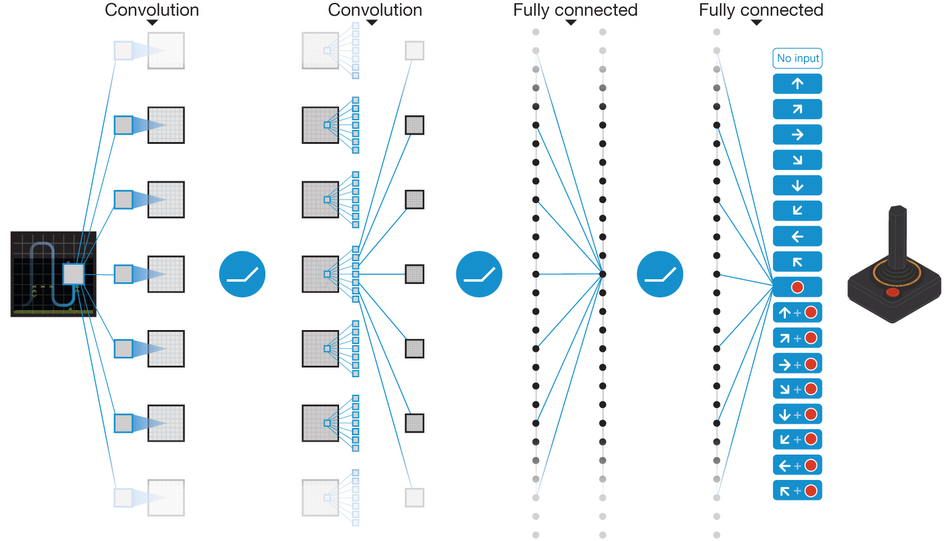
\includegraphics[width=0.7\textwidth]{Figures/TheoreticalBackground/playing_atari.jpg}
	\caption{The arhitecture of the network used in the article "Playing Atari with Deep Reinforcement Learning"}
	\label{fig:playing_atari}
\end{figure} 

This network is tested on seven Atari games, and the approach in this paper gave state-of-the-art result in six of the seven games. Finally it showed better performance than a expert human player in three out of the seven games.  

\subsection{Mastering the Game of Go with Deep Neural Networks and Tree Search}\cite{Silver_2016}
This paper introduce a new approach to compete in the classic game Go. The game of Go is the most challenging classic game for artificial intelligence, due to the enormous search space and the difficulty of evaluating board positions and moves. \\
\\
They employ a similar architecture as in \cite{DBLP:journals/corr/MnihKSGAWR13}. Here they pass in the board position as a $19 x 19$ image and use convolutional layers to construct a representation of the position. It uses neural networks to reduce the search space, this is done by use of value networks to evaluate board position and policy networks to select moves.\\
\\
training ? 
\\
By combining tree search with policy and value networks, \textit{AlphaGo} has reached a professional level in Go. In March 2016 \textit{AlphaGo} won 4-1 against the legendary Lee Sedol , the top Go player in the world over the past decade.  

\subsection{A3C 2016}
...
\subsection{Framework 2017}
...